\documentclass{article}

\usepackage[margin=1in]{geometry} 
\usepackage{amsmath,amsthm,amssymb,hyperref, multicol, TikZ, romannum}
\usetikzlibrary{arrows.meta, positioning}
\usepackage[framemethod=tikz]{mdframed}


\newcounter{result}[section]
\setcounter{result}{0}



\newenvironment{result}[4]{
  \refstepcounter{result}

  \mdfsetup{
    frametitle={
      \tikz[baseline=(current bounding box.east),outer sep=0pt]
        \node[anchor=east,rectangle,fill=#4!20]
        {\strut #1~#2.\arabic{result}:~#3};
    },
    innertopmargin=10pt,
    linecolor=#4!20,
    linewidth=2pt,
    topline=true,
    frametitleaboveskip=\dimexpr-\ht\strutbox\relax
  }

  \begin{mdframed}\relax \begin{center}
}{
  \end{center} \hfill \end{mdframed} \vspace{3\baselineskip}
}

\hypersetup{colorlinks=True, linkcolor=cyan}



\newcommand{\R}{\mathbb{R}}  
\newcommand{\Z}{\mathbb{Z}}
\newcommand{\N}{\mathbb{N}}
\newcommand{\Q}{\mathbb{Q}}

\newcommand{\suc}{\!+\!\!+\!}


\begin{document}
\pagenumbering{arabic}


\title{Tao Analysis - My Visualisations and Proofs}
\author{Rhitt C}

\maketitle
\tableofcontents
\pagebreak

\section{Abstract}

This text is heavily inspired by Terrence Tao's Analysis Vol. \Romannum{1} and \Romannum{2}.
However, I have taken many liberties in altering formulations to my liking and providing visuals.
I'm also including my solutions to the exercises for future reference.



\section{Construction of $\N$}


\subsection{Peano Axioms}

We lay our assumed axioms under the Peano construction of $\N = \{0, 1, 2, \dots\}$ as follows, 
motivated by the physical intuition of ``counting numbers". All later results, apart from definitions, must strictly follow logically from the Peano Axioms and ZFC Axioms (defined strictly in next chapter):




    We start with the bare minimum by demanding that some fixed object, namely $0$, be well defined:

    \begin{result}{Axiom}{P}{Existence of 0}{red}

        There exists an object $0$ that is natural.
        $$\exists0\quad s.t.\quad 0 \in \N \quad$$

        
\begin{tikzpicture}[scale=1.2]
            \fill[cyan] (0,0) circle (3pt);
            \draw[ultra thick, cyan] (0,-0.2) -- (0, 0.2);
            \node[below, cyan, font=\large] at (0,-0.2) {$0$};
        \end{tikzpicture}

    \end{result}



    Now to populate $\N$, we introduce a new primitive operation (that will later by superseded by addition) called \textit{succession}, with the property of closure.
    Informally, we hope that it behaves like our intuition for incrementing a number by $1$, and thus forces the infinitely many ``counting numbers" to now be well defined and in $\N$.
    Denote the succession of all $n\in\N$ as $n\suc$, and label $(1:=0\suc),\; (2:=1\suc),\; (3:=2\suc),\;\dots$


    \begin{result}{Axiom}{P}{Closure of $\N$ under $(\suc)$}{red}
        All naturals have natural successions.
        $$\forall n\in\N\quad n \in \N \implies (n\suc) \in \N$$

        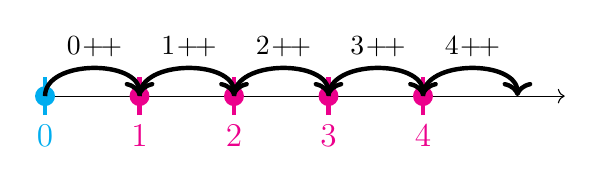
\begin{tikzpicture}[scale=1.2]

            \draw[->] (0,0) -- (5.5, 0);
            \fill[cyan] (0,0) circle (3pt);
            \draw[ultra thick, cyan] (0,-0.2) -- (0, 0.2);
            \node[below, cyan, font=\large] at (0,-0.2) {$0$};

            \fill[magenta] (1,0) circle (3pt);
            \draw[ultra thick, magenta] (1,-0.2) -- (1, 0.2);
            \node[below, magenta, font=\large] at (1,-0.2) {$1$};
            \draw[->, ultra thick] (0,0) to[bend left=90] node[pos=0.5, sloped, above] {$0\suc$} (1,0);

            \fill[magenta] (2,0) circle (3pt);
            \draw[ultra thick, magenta] (2,-0.2) -- (2, 0.2);
            \node[below, magenta, font=\large] at (2,-0.2) {$2$};
            \draw[->, ultra thick] (1,0) to[bend left=90] node[pos=0.5, sloped, above] {$1\suc$} (2,0);

            \fill[magenta] (3,0) circle (3pt);
            \draw[ultra thick, magenta] (3,-0.2) -- (3, 0.2);
            \node[below, magenta, font=\large] at (3,-0.2) {$3$};
            \draw[->, ultra thick] (2,0) to[bend left=90] node[pos=0.5, sloped, above] {$2\suc$} (3,0);

            \fill[magenta] (4,0) circle (3pt);
            \draw[ultra thick, magenta] (4,-0.2) -- (4, 0.2);
            \node[below, magenta, font=\large] at (4,-0.2) {$4$};
            \draw[->, ultra thick] (3,0) to[bend left=90] node[pos=0.5, sloped, above] {$3\suc$} (4,0);

            \draw[->, ultra thick] (4,0) to[bend left=90] node[pos=0.5, sloped, above] {$4\suc$} (5,0);

        \end{tikzpicture}
    \end{result}

    

    \pagebreak
    However, \textcolor{magenta}{P.1} and \textcolor{magenta}{P.2} alone are not strong enough to force $\N$ to populate with our infinitely many elements.
    In particular, they do not prevent existence of an $n\in\N$ with $n\suc=0$.
    And yet, informally speaking, this leads to a modulo cycle in which only $n+1$ elements exist in $\N$, and everything beyond that overflows back to $0$, like in a computer. 
    Modulo sets have many applications, but they are not what we desire as a full set of ``counting numbers'', particularly if that $n$ turns out to be $0$ itself, leading to a trivial $\N = \{0\}$.
    So we explicitly force $\N$ to not be such a modulo cycle by demanding that a natural's succession never overflows back to $0$.

    \begin{result}{Axiom}{P}{$\N$ is not a modulo cycle overflowing to $0$}{red}
        No natural's succession can be $0$.
        $$\forall n\in\N\quad (n\suc) \neq 0$$


        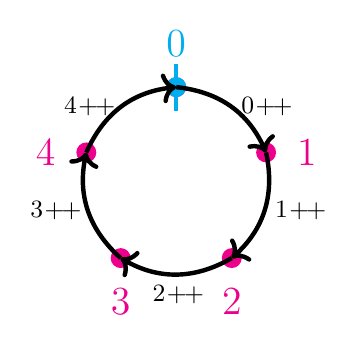
\begin{tikzpicture}[scale=1.2, every node/.style={font=\large, inner sep=1pt}]
            \def\n{5}
            \def\radius{1}

            \foreach \i in {0,...,4} {
                \pgfmathsetmacro{\angle}{90-\i*360/\n}
                \coordinate (N\i) at (\angle:\radius);
                \fill[magenta] (N\i) circle (3pt);
            }
            \fill[cyan] (N0) circle (3pt);

            \draw[ultra thick, cyan] (N0 |- 0,0.75) -- (N0 |- 0,1.25);

            \node[above=10pt, cyan, font=\Large] at (N0) {$0$};
            \node[right=10pt, magenta, font=\Large] at (N1) {$1$};
            \node[below=10pt, magenta, font=\Large] at (N2) {$2$};
            \node[below=10pt, magenta, font=\Large] at (N3) {$3$};
            \node[left=10pt, magenta, font=\Large] at (N4) {$4$};

            \draw[->, ultra thick] (N0) to[bend left=30] node[midway, right, outer sep = 1mm, font=\small] {$0\suc$} (N1);
            \draw[->, ultra thick] (N1) to[bend left=30] node[midway, right, outer sep = 1mm, font=\small] {$1\suc$} (N2);
            \draw[->, ultra thick] (N2) to[bend left=30] node[midway, below, outer sep = 1mm, font=\small] {$2\suc$} (N3);
            \draw[->, ultra thick] (N3) to[bend left=30] node[midway, left, outer sep = 1mm, font=\small] {$3\suc$} (N4);
            \draw[->, ultra thick] (N4) to[bend left=30] node[midway, left, outer sep = 1mm, font=\small] {$4\suc$} (N0);
        \end{tikzpicture}

    \end{result}


    As it stands, the issue hasn't been fully resolved yet.
    There is still the pathological case of an \textit{offset} modulo cycle, in which an $n\in\N$ overflows back so that $n \mapsto m\suc$ even though we already have a previous $m\mapsto m\suc$.
    We now complete our requirements on $(\suc)$ by demanding no such dual mappings to the same succession i.e. we make $(\suc)$ \textit{injective}.


    \begin{result}{Axiom}{P}{$\N$ has no otherwise offset modulo cycles either}{red}

        Succession is injective (one-to-one). That is, distinct naturals have distinct successions.
        $$\forall n, m\in\N\quad n \neq m \implies (n\suc) \neq (m\suc)$$

        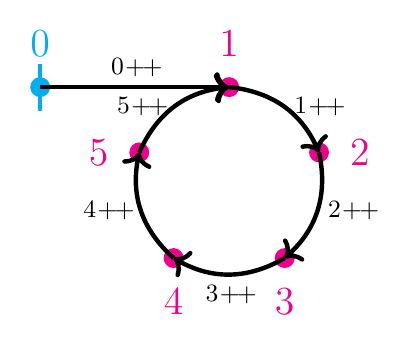
\begin{tikzpicture}[scale=1.2, every node/.style={font=\large, inner sep=1pt}]
            
            \def\n{5}
            \def\radius{1}

            \foreach \i in {0,...,4} {
                \pgfmathsetmacro{\angle}{90-\i*360/\n}
                \coordinate (N\i) at (\angle:\radius);
                \fill[magenta] (N\i) circle (3pt);
            }
            \fill[cyan] (-2, 0 |- N0) circle (3pt);
            \draw[ultra thick, cyan] (-2,0.75) -- (-2,1.25);


            \node[above=10pt, cyan, font=\Large] at (-2, 0 |- N0) {$0$};
            \node[above=10pt, magenta, font=\Large] at (N0) {$1$};
            \node[right=10pt, magenta, font=\Large] at (N1) {$2$};
            \node[below=10pt, magenta, font=\Large] at (N2) {$3$};
            \node[below=10pt, magenta, font=\Large] at (N3) {$4$};
            \node[left=10pt, magenta, font=\Large] at (N4) {$5$};

            \draw[->, ultra thick] (-2, 0 |- N0) to node[midway, above, outer sep = 1mm, font=\small] {$0\suc$} (N0);
            \draw[->, ultra thick] (N0) to[bend left=30] node[midway, right, outer sep = 1mm, font=\small] {$1\suc$} (N1);
            \draw[->, ultra thick] (N1) to[bend left=30] node[midway, right, outer sep = 1mm, font=\small] {$2\suc$} (N2);
            \draw[->, ultra thick] (N2) to[bend left=30] node[midway, below, outer sep = 1mm, font=\small] {$3\suc$} (N3);
            \draw[->, ultra thick] (N3) to[bend left=30] node[midway, left, outer sep = 1mm, font=\small] {$4\suc$} (N4);
            \draw[->, ultra thick] (N4) to[bend left=30] node[midway, left, outer sep = 1mm, font=\small] {$5\suc$} (N0);
        \end{tikzpicture}


    \end{result}


    \pagebreak 
    We now lay out by far the most useful axiom of $\N$ to handle the sheer infinite size of $\N$ recursively.
    It is induction.
    \begin{result}{Axiom}{P}{(PMI) Principle of Mathematical Induction}{red}
    
        If a proposition of naturals is met for $0$ (Base Case), and it being satisfied for some natural implies it's met for the succession as well (Inductive Case), then as a domino effect, then the proposition is met for all naturals.

        \hfill

        $\forall P:\N\to \{\text{True}, \text{False}\}\qquad(P(0)\;\&\;(\forall k\in\N)P(k)\!\!\implies\!\!P(k\suc)) \quad \implies \quad \forall n\in\N \quad P(n)$

        \vspace{2\baselineskip}

        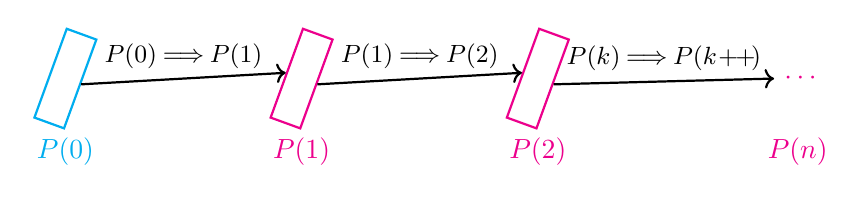
\begin{tikzpicture}[
            dom/.style={rectangle, draw, rotate=-20, minimum width=0.4cm, minimum height=1.2cm, thick},
            arrow/.style={->, thick}
        ]

            \node[dom, cyan] (D1) at (0,0) {};
            \node[below=18pt, cyan] at (D1) {$P(0)$};

            \node[dom, magenta] (D2) at (3,0) {};
            \node[below=18pt, magenta] at (D2) {$P(1)$};

            \node[dom, magenta] (D3) at (6,0) {};
            \node[below=18pt, magenta] at (D3) {$P(2)$};

            \node[below=18pt, magenta] at (9.3, 0) {$P(n)$};


            \draw[arrow] (D1.east) -- node[midway, above, font=\small] {$P(0)\!\!\implies\!\!P(1)$} (D2.west);
            \draw[arrow] (D2.east) -- node[midway, above, font=\small] {$P(1)\!\!\implies\!\!P(2)$} (D3.west);
            \draw[arrow] (D3.east) -- node[midway, above, font=\small] {$P(k)\!\!\implies\!\!P(k\suc)$} (9, 0) node[magenta, right] {$\cdots$};

        \end{tikzpicture}

    \end{result}

    Abstractly speaking, any other set $X$ equipped with an analogous operation $S: X\to X$ that obeys the 5 Peano Axioms is said to be \textit{isomorphic} with $\N$, denoted $X\cong\N$.
    Note that due to our later discussions only relying on logical implications from the axioms, which are met by $X$, the results we derive must also apply to $X$.

    \subsection{Addition}
    \subsection{Multiplication}

\end{document}